\chapter{Passive Haptics Experiment}
\label{chap:ph_exp}

The first experiment, described in the previous chapter, provided validation that the R3C technology could be used for interacting with a non-functioning mockup.
We found that subjects had a near-perfect success rate using the hand tracking sensor to activate buttons, with accuracy comparable to their performance in a non-virtual environment.
There was a difference in time, with the subjects performing faster in the real, non-virtual environment, and slower in all the virtual environment conditions.
One of the unanswered questions was the effect of the panel as passive haptics on the movement time and accuracy.
The difference in movement time between the subjects using the passive haptics and those without were insignificant.
The main focus of this experiment is the independent variable of passive haptics.
The experimental conditions are reduced from the last experiment to just two: one with passive haptics and one without.
Both conditions are performed with the use of the head-mounted display and the hand tracker.
A more thorough examination of movement time and accuracy is provided by the use of Fitts' Law, and additional dependent measures are also investigated, including presence, learning rate, and trajectory metrics.
This experiment aims to provide a more complete understanding on how the use of passive haptics affects the interaction of a subject with a virtual cockpit panel.
A version of this chapter was presented at the 2017 AIAA Modeling and Simulation Technologies \citep{joyce_passive_2017}.

\section{Introduction}

Passive haptics is a term that has been used to describe a variety of technologies or techniques to provide the sense of touch to a user of a virtual environment.
It is often defined by its distinction from active haptics, which simulate the sense of touch with energy exchange, typically electromechanical.
A common active haptic technology used in immersive virtual environments is a haptic glove, which utilizes small motors at the fingertips.
In contrast, passive haptics often utilize proxy objects placed in the physical world to co-incide with the virtual environment experience.
The proxy objects can be simple or complex.
They can be colocated and accurate with the virtual world or purposefully designed to trick the user.
In our paper, we utilize a simple colocated passive haptic device and measure its effect on the presence and performance of subjects using a 2D panel in a 3D immersive virtual environment.

The advantages to using a simple passive haptic can be easily understood: less cost and complexity compared to most active haptic solutions.
However, the disadvantage comes with its inflexibility.
Due to their nature, passive haptics often have to be purpose built for a single or limited experience.
While past research has aimed to address this, by either actively positioning a proxy object or simplifying the proxy object to fool the user, our application suffers only minimally from this limitation.
The motivation for our research comes from the application of designing aerospace cockpits, complex human-machine interfaces where the user is stationed at their workspace.
For the purpose of evaluating a cockpit design, the user does not need a dynamic tactile environment.
Furthermore, many cockpit design processes already create a physical mockup which can provide the passive haptics for this evaluation.

We present our findings in testing passive haptics versus no haptics in an immersive virtual reality environment.
Using a head-mounted display and a hand tracker, the subjects performed the same Fitts' Law style task under these two haptic conditions.
The passive haptics was a flat surface placed at an angle on a desk in front of their seating area.
Their performance on the Fitts' task was recorded as well as their responses to a presence survey, a self reported arm fatigue score and a general questionnaire.

\section{Background}

In this section, a brief summary of the relevant topics is given.
A more thorough treatment of the background is in Chapter~\ref{sec:intro_background}.

\subsection{Passive Haptics}

Passive haptics have seen limited, but promising results in research.
\citet{insko_passive_2001} had subjects navigate a maze in a virtual environment.
They found that subjects reported increased presence using passive haptics, and also found that subjects trained with the passive haptics performed better after they were removed than a control group that never used passive haptics.
\citet{borst_evaluation_2005} created a `mixed haptics' system, combining active haptic gloves with a physical panel for passive haptics.
Again, performance was increased with the haptics, but minimal differences were found between using the mixed haptics and the passive haptics alone.
\citet{kohli_redirected_2012} performed a Fitts' Law evaluation of passive haptics, but did not compare to a no haptics condition.
Similar to our motivation and work, \citet{schiefele_simple_1998} replaced a cockpit panel with a flat panel in an immersive head-mounted virtual environment, and found that users could activate buttons and switches in less time with the panel present than without.
We build on this previous work by investigating the effects of passive haptics with the latest virtual environment technology, as well as performing a complete Fitts' Law characterization between no haptics and passive haptics.

\subsection{Fitts' Law}

Fitts' Law is a well established model of human movement that has been used extensively to measure the performance of input devices.
We use the Fitts' throughput in this experiment to compare our experimental conditions.
Throughput ($\mathrm{TP}$) is defined as:
\begin{equation}
    \mathrm{TP}=\frac{\mathrm{ID}}{\mathrm{MT}}
    \label{eq:throughput}
\end{equation}
where $\mathrm{MT}$ is the movement time and $\mathrm{ID}$ is the index of difficulty.
Index of difficulty is a property of the geometry of the targeting movement, combining the distance to the target from the starting location ($D$) and the width of the target ($W$).
We use the Shannons' formulation of index of difficulty:
\begin{equation}
    \mathrm{ID}=\log_2\left(\frac{D}{W}+1\right)
%    \label{eq:index_of_difficulty}
\end{equation}
The index of difficulty has units of bits, and the throughput has units of ``bits per second'' (\si{\bps}).
Throughput can be thought of theoretically as the amount of information (`bits') the human can input with the particular input device or method per time (`per second').
A higher throughput indicates that humans are able to use the input method more accurately and more quickly.

In this experiment, we use the ISO 9241-9 ``Fitts' circle'' standard (Figure~\ref{fig:ph_fitts_circle}).
The adjustment for accuracy \citep{welford_fundamentals_1968} is used to calculate the effective width.
The effective width, $W_e$, performs a correction for the performance of the subject based on the end point positions on the target for all their movements.
The effective width is calculated as $W_d=4.1\sigma$, where $\sigma$ is the standard deviation of the endpoint positions.

\begin{figure}
    \centering
    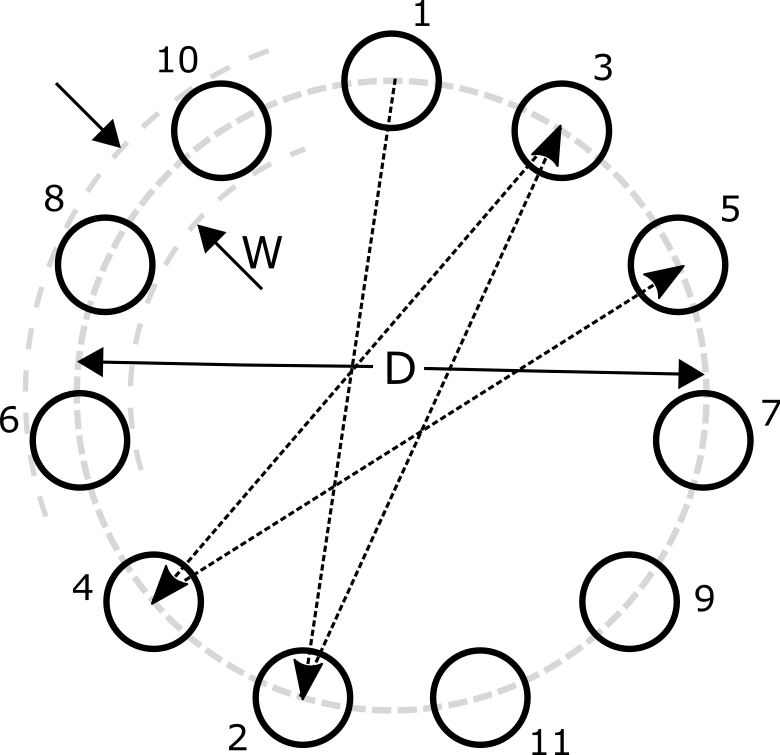
\includegraphics[width=3in]{fitts_circle.png}
    \caption{Fitts' Circle diagram. $D$ is the distance between targets and $W$ is the width of the targets.}
    \label{fig:ph_fitts_circle}
\end{figure}

Previous work of evaluating virtual environments and input devices with Fitts’ Law mostly consist of evaluating 3D tasks \citep{chun_evaluating_2004,liu_comparing_2009,teather_evaluating_2010}.
\citet{kohli_redirected_2012} used a passive haptic environment with a head-mounted display, but evaluation focused on their warped virtual space technique.
Recently, some reports have evaluated the Fitts’ performance of the LeapMotion hand tracker \citep{coelho_pointing_2014,seixas_one_2015}, but none have combined hand-tracking with the use of a head-mounted display.

\subsection{Presence}

The feeling of presence is often specified as a goal of a virtual environment.
A definition from \citet{witmer_measuring_1998} reads:
\begin{displayquote}
\textit{Presence} is defined as the subjective experience of being in one place or environment, even when one is physically situated in another.
\end{displayquote}
%\citet{sheridan_musings_1992} argued that presence is a subjective sensation that necessitates a subjective measure.
Increased presence has been shown to lead to increased performance in a virtual environment task \citep{youngblut_relationship_2003}.
We use a version of the Presence Questionnaire (PQ) proposed by \citet{witmer_measuring_1998}.
The post-questionnaire consists of 16~questions with a seven-point Likert scale.
\citet{nystad_comparison_2004} found the PQ to be sensitive to technology and interaction methods, so it was chosen to investigate the differences between the two conditions.

\subsection{Arm Fatigue}

Despite the concern of arm fatigue in virtual environments \citep{burdea_virtual_2003}, it was surprising that most results in literature were anecdotal or for mitigation without quantification of the fatigue.
%Since fatigue is a subjective quantity, it can be hard to measure it between subjects, and sometimes even within.
%The negative impact of arm fatigue on using virtual environments makes it worth investigating.
The arm fatigue scale used within this experiment is the Borg Rating of Perceived Exertion (RPE) scale that ranges from \numrange{6}{20} \citep{borg_borgs_1998}.
\citet{hincapie-ramos_consumed_2014} proposed a model for quantifying and predicting the amount of arm fatigue that correlated well with a Borg scale.
Although there does not exist a standard for arm fatigue measurements in virtual environments, we hope that future researchers will consider including arm fatigue ratings in their experiments.

\section{Methods}

The purpose of the experiment described within this paper is to answer the following research questions:

\begin{enumerate}
    \item Do subjects learn the task more quickly with passive haptics?
    \item Is the Fitts' throughput higher with passive haptics?
    \item What are the differences between the formation of reaching motion trajectories with passive haptics?
    \item Do subjects report less arm fatigue with passive haptics?
    \item Do subjects feel more presence with passive haptics?
\end{enumerate}

\subsection{Experimental Setup}

For the experimental setup, subjects were seated at a desk with a blank panel mounted at an angle in front of them.
The plywood panel (square with length of \SI{18}{\inch}) was used to provide only the backstop of the virtual buttons for the ``Passive Haptics'' condition.
The button selection is registered by the subject moving their index finger into a detection zone (cylinder for the circle buttons) in front of the button that extends outward \SI{0.5}{\inch}.
Their entrance into the hover zone is indicated to them by the button changing color.
A successful button press is registered after \SI{150}{\milli\second}, and is indicated by the color turning off and a button click noise being played over speakers.

The equipment used consists of an Oculus Rift DK2 (Development Kit 2) head-mounted display (HMD) and a LeapMotion hand tracker.
The low-persistence OLED display of the HMD has a resolution of 1920x1080, with a refresh rate of \SI{75}{\hertz}.
The field of view is approximately \ang{100}.
It utilizes internal sensors (accelerometers and gyros) and an external infrared camera for head tracking.
The configuration and calibration of the LeapMotion hand tracker is described in Chapter~\ref{sec:proto-hand-tracking}.

\subsection{Experimental Task}

The experimental task was a Fitts' circle in the virtual environment, performed by subjects in two haptic conditions.
The subjects were seated at a desk for the experimental task, and the circle was located on a panel mounted on the desk.
The two haptic conditions were ``No Haptics (NH)'' and ``Passive Haptics (PH).''
These conditions are pictured in Figure~\ref{fig:ph_conditions}.
For the ``Passive Haptics'' condition a physical panel was co-located with the panel in the virtual world, and it was removed for the ``No Haptics'' condition.

\mbox{}\hfill
\begin{figure}
    \centering
    \begin{subfigure}[t]{0.3\linewidth}
        \centering
        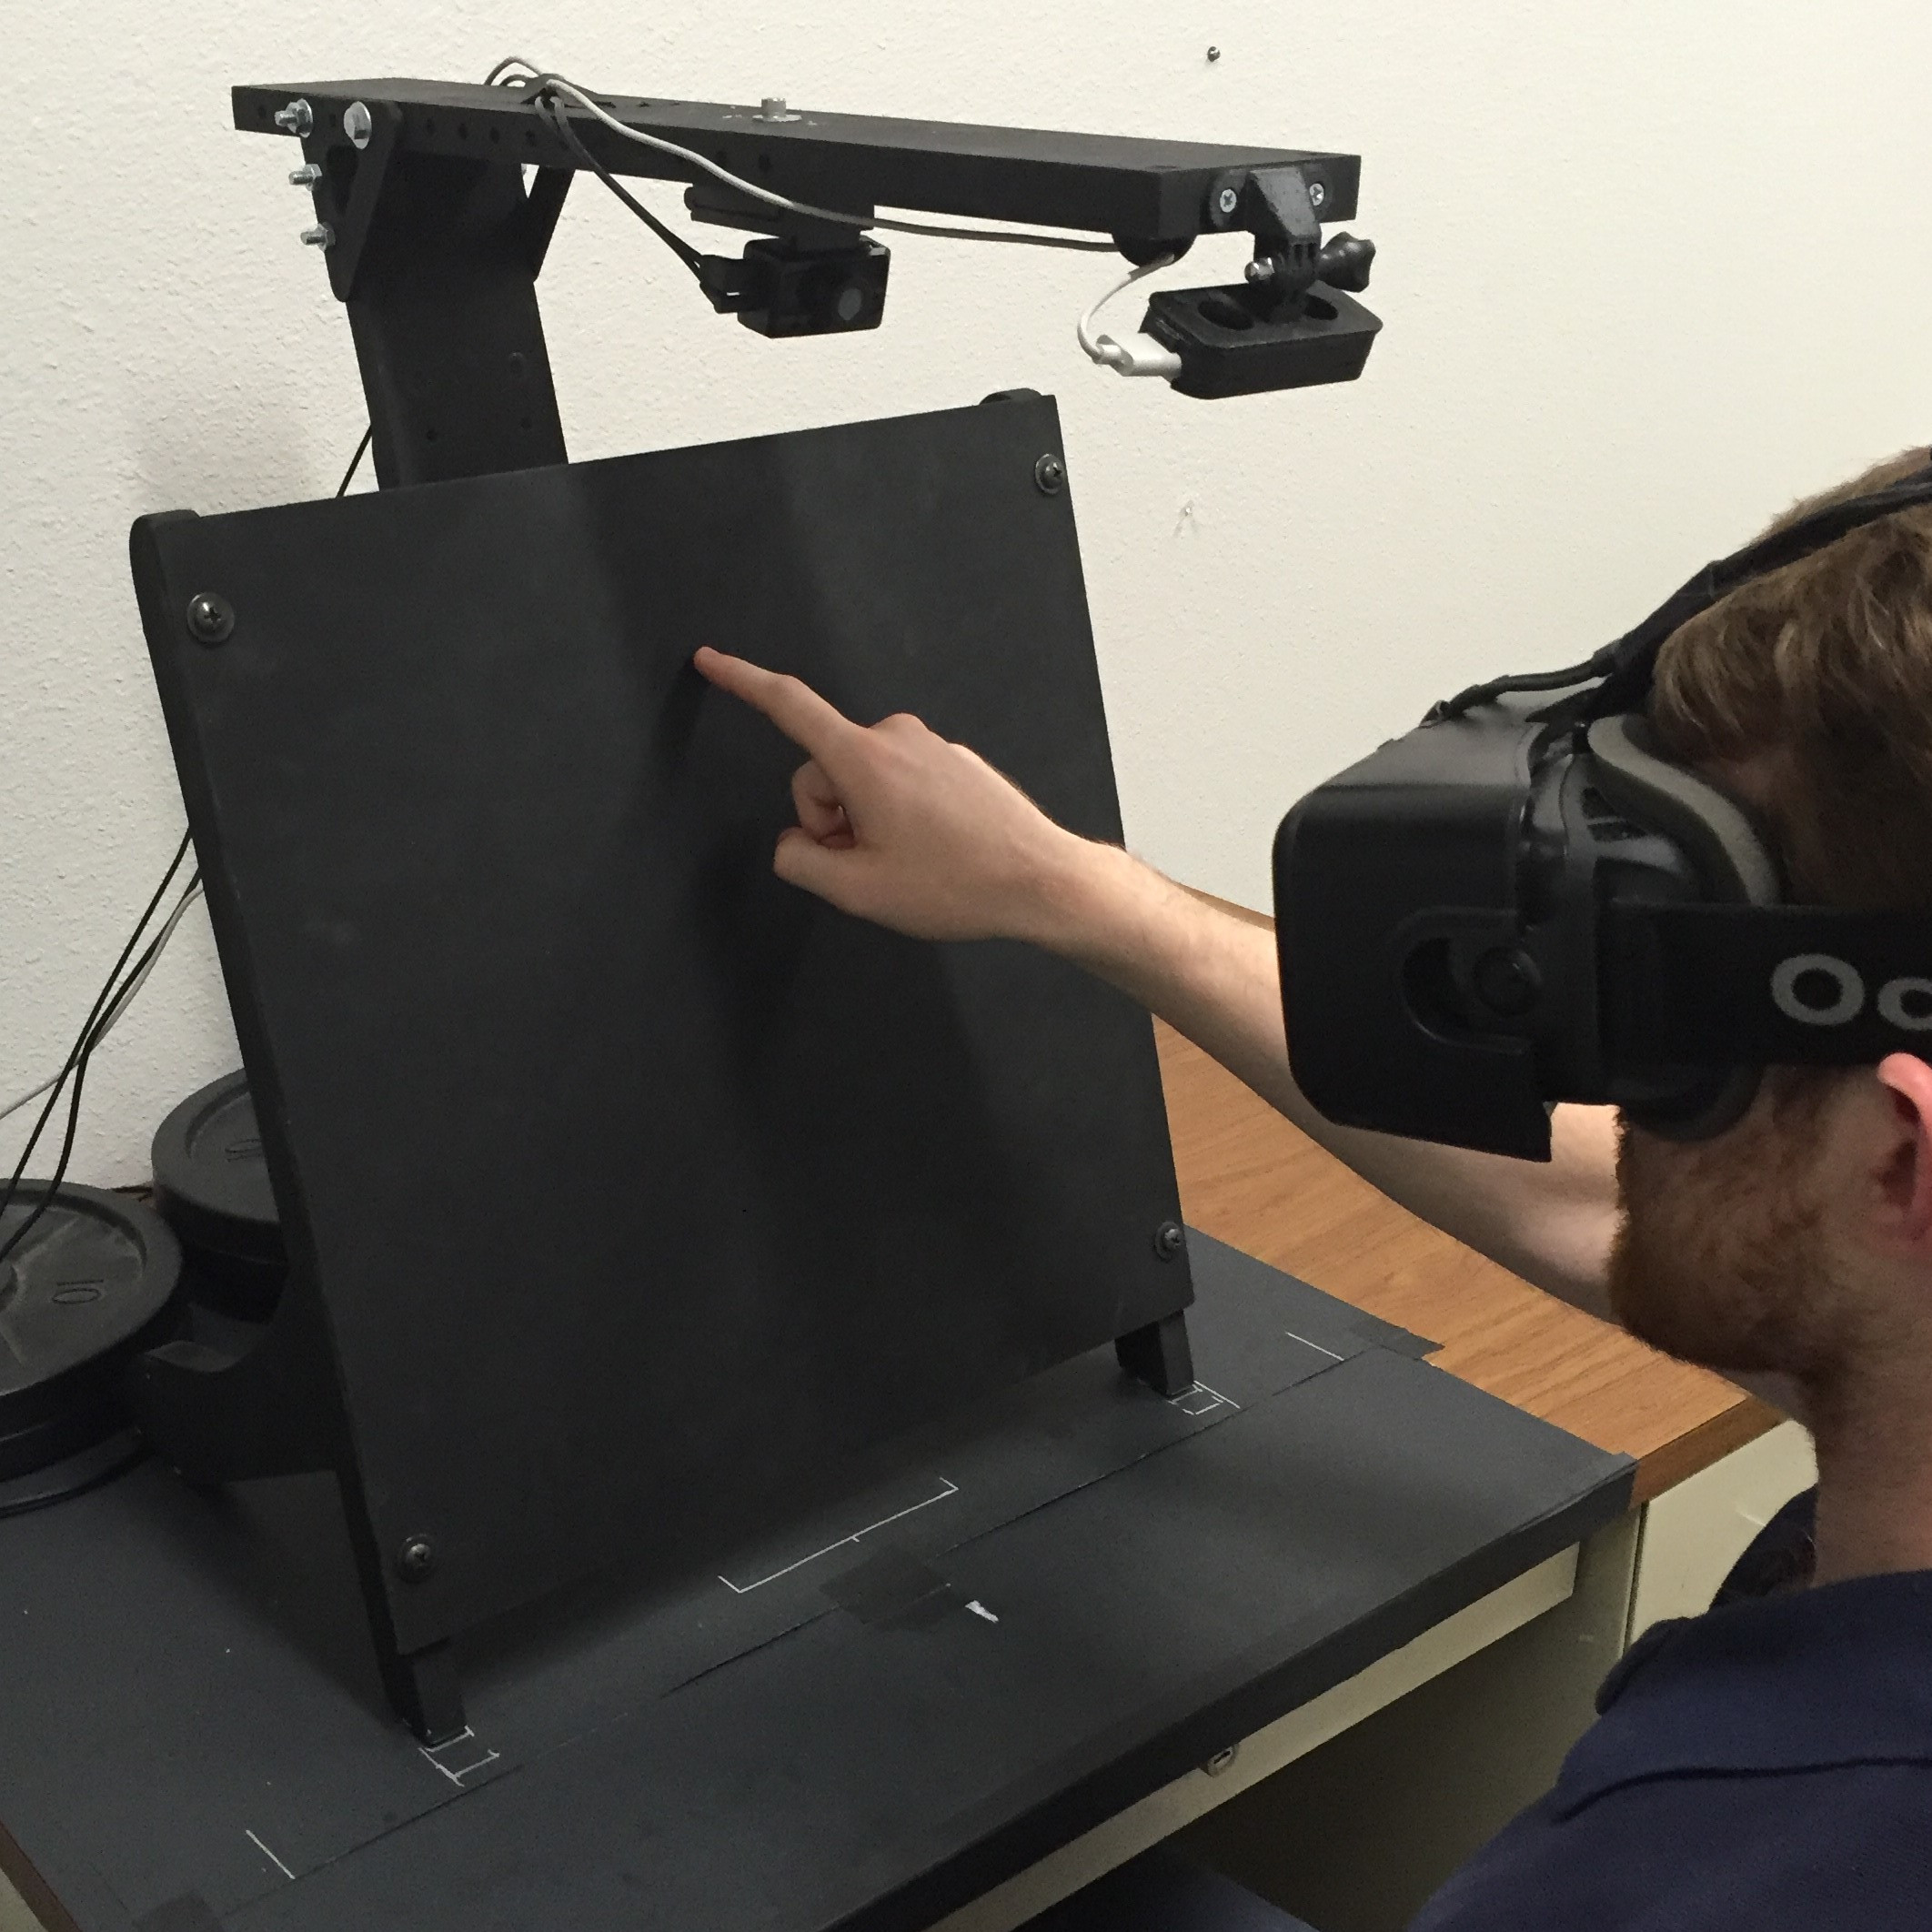
\includegraphics[width=0.9\linewidth]{ph_ph_condition.jpg}
        \caption{Passive Haptics condition (PH)}
        \label{fig:ph_conditions:ph_condition}
    \end{subfigure}\hfill
    \begin{subfigure}[t]{0.3\linewidth}
        \centering
        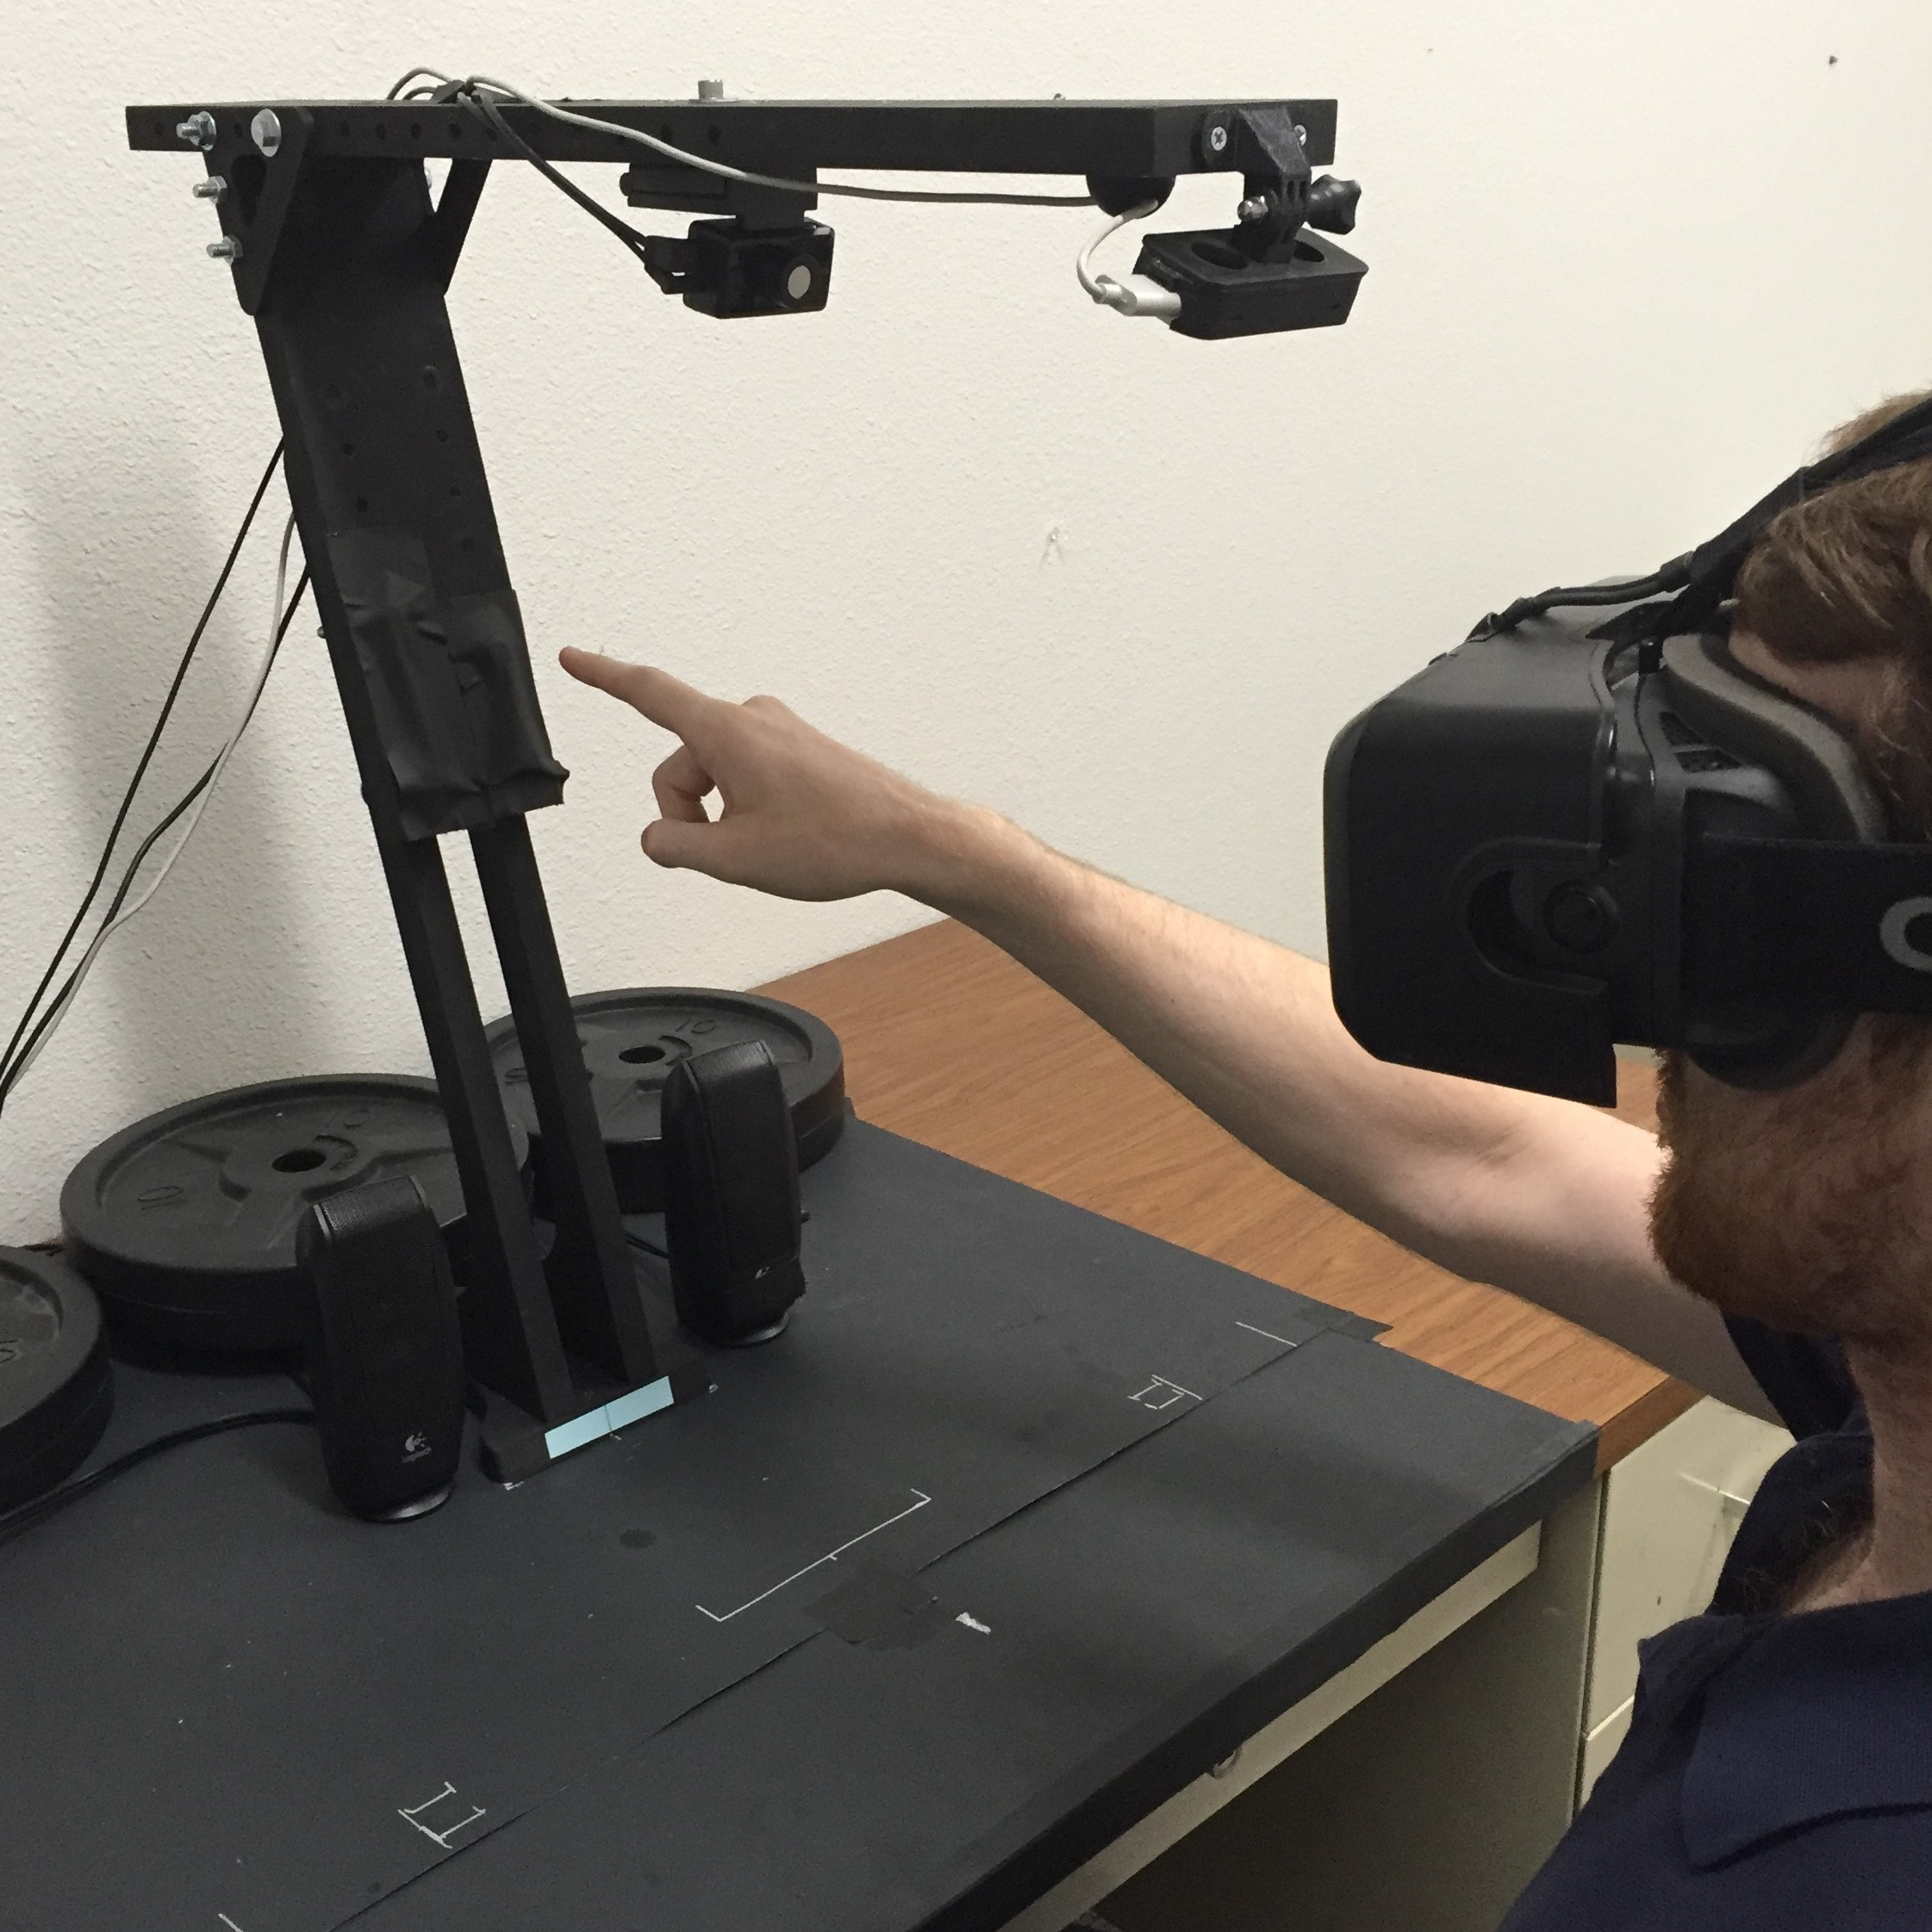
\includegraphics[width=0.9\linewidth]{ph_nh_condition.jpg}
        \caption{No Haptics condition (NH)}
        \label{fig:ph_conditions:nh_condition}
    \end{subfigure}\hfill
    \begin{subfigure}[t]{0.3\linewidth}
        \centering
        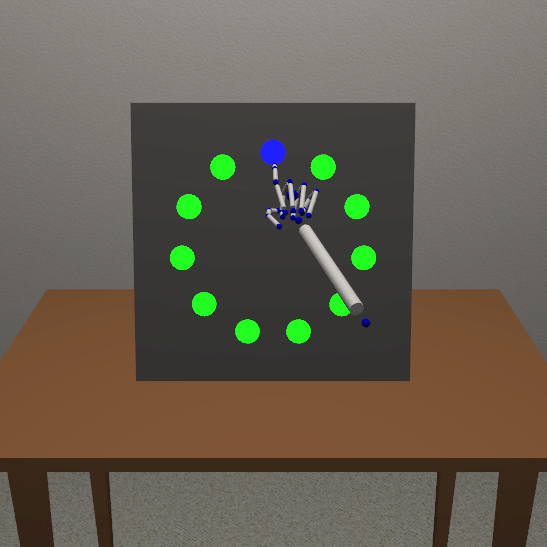
\includegraphics[width=0.9\linewidth]{ph_virtualview.png}
        \caption{View of virtual world (same for both)}
        \label{fig:ph_conditions:virtual}
    \end{subfigure}
    \caption{Experimental conditions and view of virtual environment.}
    \label{fig:ph_conditions}
\end{figure}
\hfill\mbox{}

With the two haptic conditions, there were no differences in the task itself or in the method of button activation.
The only difference between the conditions was the removal of the physical panel.
The hand tracker remained in the same location, preserving the location of the buttons in the virtual environment.
The dimensions of the virtual world were no different for either condition.
In fact, there was no change to the software between the conditions.

Subjects performed the Fitts' circle for three different distances (\SIlist{20;30;40}{\centi\meter}) and five different button widths (\SIlist{5;10;15;20;25}{\milli\meter}).
These configurations were chosen to span a wide range of indices of difficulty (\numrange{3.2}{6.4}).
For each configuration of distance and width, subjects had to complete the full pattern of 11 buttons three times consecutively.
This set of 30 movements\footnote{10 movements between the 11 targets.} for a single configuration is referred to as a single trial for a subject.
The distance was kept constant for the consecutive trials until all five button widths were complete.
The distances were presented in either smallest to largest or vice versa, which was counterbalanced among subjects.

This set of 15 trials was repeated for each haptics condition and the order was kept the same within subjects.
The sequence that the two conditions were presented to each subject was also counterbalanced.
The dependent measures were tested for interaction with sequence to determine if the results had a condition order effect.

\subsection{Experiment Design}

As described in the previous section, the experiment was performed with a within-subjects design.
Subjects were asked to complete the same experimental task for both conditions of haptics: Passive Haptics (PH) and No Haptics (NH).
The two different haptic conditions are the main independent variables.

We expected significant skill transfer between the two conditions, so the order in which subjects performed the two conditions was counterbalanced.
This created a second independent variable that is between subjects.
The subjects who performed the conditions with the PH being their first condition were one group, and the subjects who performed NH as their first condition were a second group.
We call this grouping ``sequence'' and refer to the two groups as ``PH First'' and ``NH First''.

For a Fitts' Law evaluation, it is often recommended that the data collection only begins when the subject is fully trained on the task.
However, one of the goals of the experiment is to investigate the learning rate of the subjects.
For that reason, the subjects were given no separate training time for the task or virtual environment.
In lieu of collecting the data from fully trained subjects, the throughput analysis will be carried out on movements that are determined to be composed of mostly ballistic motion.
The filtering parameters were determined post-hoc from the trajectory recordings.
Their development and parameter selection are discussed in the results.

\subsection{Dependent Measures}

The main dependent measure is the Fitts' throughput, measured through the movement time between button presses.
Additionally, the trajectory of each movement is recorded from the hand tracker for analysis.
To determine the arm fatigue, subjects were asked to rate their arm fatigue on the Borg scale from \numrange{6}{20}.
The scale was presented with anchors as shown in Appendix~\ref{sec:app_ph_exp} (Table~\ref{tab:ph_borg_scale}).
The arm fatigue rating was collected at the beginning of each condition, and then after every other configuration of distance and width combination (and after the final trial due to an odd number of trials).
At the completion of each condition the subject was given a presence questionnaire.
At the end of the experiment, an additional condition comparison survey was given to ask for opinions on the two haptic conditions.

\subsection{Trajectory Phases}
\label{sec:ph_traj_phases}

Human reaching movements have long been known to consist of two distinct phases \citep{woodworth_accuracy_1899}: a ballistic phase and a corrective phase.
The ballistic phase is an open-loop, gross adjustment towards the target, while the corrective phase is more refined movement honing in on the target.
To separate the trajectories into the various phases, a simple algorithm was developed.
First, the local minima are found throughout the velocity profile of the movement to separate the movement into various submovements.
The ``ballistic phase'' is then classified as the submovement which contains the peak velocity of the entire movement.
The various submovements after the ballistic phase are classified as the ``corrective phase''.
Any movement before the ballistic phase is classified as a ``reaction time''.
An example of the results of this classification is shown in Figure~\ref{fig:ph_trajectory_ballistic}.
This mathematical definition does break down for certain cases where a subject might have two submovements in the ballistic phase due to a mid-course correction or similar, however one of the main purposes of this classification for this experiment was to find movements which are appropriate to use for the Fitts' Law calculations.
Therefore, movements with multiple submovements are likely to not be ballistic, well-learned movements.


\begin{figure}
    \centering
    \includegraphics[width=4.0in]{{trajectory_velocity.ballistic}.png}
    \caption{Example trajectory with three phases indicated.}
    \label{fig:ph_trajectory_ballistic}
\end{figure}

\subsection{Trajectory Filtering}

We used a low-pass filter on the trajectory recordings to reduce the amount of noise.
The LeapMotion processes data at a variable frequency, thus creating a variable rate for recording.
The frequency typically varies from about \SI{100}{\hertz} to \SI{120}{\hertz}.
To perform the filtering, the data was first resampled to a fixed rate of \SI{100}{\hertz}.
The filter used is a fourth-order Butterworth filter with a cut-off frequency of \SI{5}{\hertz}.
The cut-off frequency was chosen as voluntary hand movements have been shown to be below such a rate \citep{riviere_toward_2003}.

\section{Results}

\subsection{Participants}

Twenty (20) subjects were recruited from the UC Davis engineering student population, both undergraduate and graduate students.
The age range was \numrange{19}{29} ($M=23.0, \sigma=3.0$) with 16 males and 4 females.
The genders were balanced among the counterbalanced sequence groups.
The total time spent in the experiment was under one hour, with a range of approximately ten to twenty minutes performing each of the two conditions in virtual reality.
Prior to the experiment, all subjects indicated either no prior experience with virtual reality or less than one hour of use of virtual reality.

\subsection{Throughput}

The throughput is calculated per movement using Equation~\ref{eq:throughput} and averaged by trial before being averaged by subject and condition.
Throughput is used to investigate the first two research questions: do the subjects learn more quickly and does their throughput performance improve with passive haptics?
We first present the learning rate results, but before the effect of throughput performance on passive haptics is reported, our data reduction methods are discussed.

\subsubsection{Rate of Learning}

\begin{figure}
    \centering
    \includegraphics[width=\textwidth]{{throughput_trials.8.0x4.0}.png}
    \caption{Throughput per trial. The learning curve exponential fit is given by Eq.~\ref{eq:ph_learning} with parameters from Table~\ref{tab:ph_tp_regression}. Error bars are standard error of the mean. Each line represents one of the counterbalanced sequence groups (those who did NH as their frist condition versus those who did PH as their first condition).}
    \label{fig:ph_throughput_trials}
\end{figure}

The average throughput for each trial, separated by haptics condition, is shown in Figure~\ref{fig:ph_throughput_trials}.
The two lines represent the counterbalanced sequence groups.
For the first condition (the first 15 trials), the NH First group performed the No Haptics condition before switching to the Passive Haptics condition for the remaining trials.
An exponential rise to a learned state is fit to each haptics condition to model the learning curve of the subjects.
The equation used is given as:
\begin{equation}
    \mathrm{TP}(T) = \mathrm{TP}_{\infty} - (\mathrm{TP}_{\infty}-\mathrm{TP}_0)e^{\left( -T / \tau \right)}
    \label{eq:ph_learning}
\end{equation}
where $T$ is the trial number, $\mathrm{TP}_{\infty}$ is the asymptotic learned value of throughput, $\mathrm{TP}_0$ is the initial value at $T=0$ and $\tau$ is the time constant.
The time constant is defined as the number of trials for the throughput to rise 36\% of the difference between the fully learned throughput ($\mathrm{TP}_{\infty}$) and the initial throughput ($\mathrm{TP}_0$).
The parameters of the fit for each condition is shown in Table~\ref{tab:ph_tp_regression}, as well as the standard error of the estimate (SEE).
The value of throughput from the regression fit as a percentage of the fully learned value ($\mathrm{TP}_{\infty}$) for representative trials are listed in Table~\ref{tab:ph_tp_regression_values}.

The rate of learning is very similar among both groups in the first condition.
For the first condition it can appear that the subjects performing NH learned more quickly than their counterparts performing PH by looking at the time constants.
However, as the values in Table~\ref{tab:ph_tp_regression_values} show, the NH First group started their first trial at a lower percentage of their final throughput value.
Both groups reached approximately 90\% of their fully learned state by the 5\textsuperscript{th} trial.
This means that the NH First group had a bigger change in performance in the first 5 trials, but both groups reached their learned state by the same trial.

The learning curves are quite different for the second condition.
The NH condition does not have a learning curve at all, with a straight line being a better fit than the exponential function.
This indicates the transfer of training from the PH condition allowed the group who did PH first to immediately perform in NH at the same level as the fully learned state of the subjects who learned NH in their first condition.
This transfer of training to the second condition did not occur as strongly for the group who did NH first.
Their initial performance of PH did start out at a slightly higher level than the subjects who did PH first (\SI{2.8}{\bps} vs \SI{2.4}{\bps}), but after 5 trials this difference had converged (\SI{3.6}{\bps} vs \SI{3.7}{bps}).

\begin{table}
    \centering
    \includetable{throughput_regressions.tex}
    \caption{Exponential fit parameters of Eq.~\ref{eq:ph_learning}. Curves are shown in Figure~\ref{fig:ph_throughput_trials}. $\mathrm{TP}_{\infty}$ is the asymptotic learned value of throughput. $\mathrm{TP}_0$ is the initial value at trial~0. $\tau$ is the time constant of the exponential function. SEE is the standard error of the estimate for the fit. Sequence refers to the counterbalancing order group. Condition indicates the temporal order. Haptics is the haptic used for that condition.}
    \label{tab:ph_tp_regression}
\end{table}

\begin{table}
    \centering
    \includetable{throughput_regression_values.tex}
    \caption{Percentage of fully learned state for various trials for each group and condition from learning model fit. $\mathrm{TP_i}$ is $\mathrm{TP}(i)/\mathrm{TP}_{\infty}$ using Eq.~\ref{eq:ph_learning}. Trial 15 is the final trial for each condition. Sequence refers to the counterbalancing order group. Condition indicates the temporal order. Haptics is the haptic used for that condition.}
    \label{tab:ph_tp_regression_values}
\end{table}

These results indicate that subjects did not learn faster with Passive Haptics.
The only differences between learning rates is the positive transfer of training from performing Passive Haptics first followed by No Haptics second.
The answer to the first research question \textit{Do subjects learn the task more quickly with passive haptics?}\ appears to be that the passive haptics does not make subjects learn faster, but they are able to learn the task more quickly without passive haptics afterward.
It does appear that the fully learned state is different between the haptic conditions, which is investigated through the use of throughput after discussing data filtering.

\subsubsection{Ballistic Movement Filtering}
\label{sec:ph_ballistic_filter}

Before they could be used for the Fitts' Law analysis, the trajectories were filtered so that only movements which were direct to target were included.
A well-learned movement appropriate for Fitts' Law is one which moves directly towards the target and does not have much extraneous movement or idle time beyond what is required to complete the task.
As a result of the experiment design and research questions requiring subjects to learn the task during the data collection, we expected many of the movements to deviate from a well-learned movement.
A number of common reasons for deviation were observed during the experiment and post-hoc examination of the dataset.
These reasons are the basis of the three filters described below.
They include undershooting the target, extra movement away from the target after the ballistic portion, and time spent not moving.
The goal of this filtering is to produce a dataset that only includes the direct to target movements appropriate for a Fitts' Law analysis for the final throughput calculations.
We describe in this section the three metrics developed based on these observed deviations that were used to determine whether a movement was direct to target.

The first metric was the ratio of path distance traveled in the ballistic phase to the distance between the targets for that movement (i.e.\ \SIlist{20;30;40}{\centi\meter}).
Ideally, the ballistic portion would cover the majority of the distance between the targets.
A movement which covered too little of the target distance could mean the subject slowed or stopped in the middle of movement, and one that covered more could mean the subject overshot or had an indirect trajectory.
A sample movement that gets flagged by this filter is shown in Figure~\ref{fig:ph_traj_filter_target}, which has a ratio of 1.49.
This is an example of a movement that does seemingly have a direct movement toward the target, but includes a large deviation perpendicular to the movement axis.
This deviation could mean the subject initially aimed their ballistic portion in the wrong direction but performed a correction during the movement.
The limits for this filter were chosen as having a ratio between 0.90 and 1.10, i.e.\ within 10\% of the target distance.
This filtered out 4577 of the 17970 movements (25.5\%).

\begin{figure}
    \centering
    \includegraphics[width=4.0in]{{trajectory_both.bad_target_filter}.png}
    \caption{An example of a movement with a large ballistic distance to target distance ratio. The bottom plot shows the projection of the trajectory on the plane of the Fitts' circle.}
    \label{fig:ph_traj_filter_target}
\end{figure}

The second filtering metric was also based on the ballistic phase path distance.
For this metric the ballistic phase path distance was compared to the total path distance the subject traveled for their entire movement.
This filter targeted movements where, after the ballistic phase, the subject moved away from the target, or had a smaller but significant movement before the main ballistic movement.
An example is shown in Figure~\ref{fig:ph_traj_filter_distance} which shows a movement which passed the first metric (the ballistic phase distance ratio to the target distance was 1.03), but the ballistic phase was only 56\% of the total distance traveled during that movement.
This was a common problem where a subject would have a false start for the next target and move away from the current target before their button press was activated.
The threshold for the filter was set at 0.80, which rejects 4264 movements that are lower than the threshold.
Of the rejected movements, only 1675 were unique from the rejected movements of the previous target distance filter.
Between the two filters so far, there have been 6252 of the 17970 movements filtered out (34.8\%).

\begin{figure}
    \centering
    \includegraphics[width=4.0in]{{trajectory_both.bad_distance_filter}.png}
    \caption{An example of a movement with a small ballistic distance to total path distance ratio. The bottom plot shows the projection of the trajectory on the plane of the Fitts' circle.}
    \label{fig:ph_traj_filter_distance}
\end{figure}


The last filter took a time based approach, and looked at the ratio of the time spent in the ballistic phase over the total movement time.
This filter removed movements where the subject spent an inordinate amount of time either before or after the ballistic phase.
If they were not moving during the non-ballistic phases, it would not have been caught by the distance-based filters either.
The threshold of 0.40 meant that 4496 movements were filtered, however only 873 of those are unique of the other two filters.
Figure~\ref{fig:ph_traj_filter_time} illustrates a movement where the subject waited before initiating the ballistic movement.
Since the subject did not move during this idle time, the other two filters did not flag this movement.

\begin{figure}
    \centering
    \includegraphics[width=4.0in]{{trajectory_both.bad_time_filter}.png}
    \caption{An example of a movement with a small ballistic time to total time ratio. The bottom plot shows the projection of the trajectory on the plane of the Fitts' circle.}
    \label{fig:ph_traj_filter_time}
\end{figure}

The combination of these three filters flags 7125 of 18000 movements as non-ballistic.
This leaves 60.4\% of the movements to be included in the ballistic movement dataset.
For each of the metrics, the threshold was determined by investigating the distribution and looking at sample movements on either end of the threshold to determine if it was an appropriate value.
The histograms of these metrics across all movements are shown in Appendix~\ref{sec:app_ph_metrics}.
The major conclusions in the following sections do not change with different choices in the thresholds (i.e.\ the statistical effects are not sensitive to the threshold choices).
%However, the use of these filters provides a

The final check before performing the Fitts' calculation was to ensure that each trial had enough data for the adjustment for accuracy calculation.
The adjustment for accuracy is based on the distribution of endpoint data from a single trial (which is one distance and width configuration).
One trial consists of 30 consecutive movements, but the ballistic filtering could diminish the amount remaining in each, so a trial was only included if at least half (15 of 30) of the movements were considered to be good movements by the ballistic filters.
This means that movements from a trial that did not have enough good movements were also filtered out from the Fitts' calculation.
Not only is this important to make sure the adjusted width is valid, it also removes trials where the subject likely did not reach a fully learned state, as most of their movements were not primarily ballistic movements direct to target.
On average, 11 of 15 trials per condition from each subject ($M=10.98, \sigma=3.25$) had enough good movements to be included.
This left 9218~movements for the Fitts' calculation, just over half of the total movements (51.3\%).
Slightly more movements were filtered from the No Haptics condition, with 47.1\% of NH movements left after the filtering, compared to 55.5\% of the PH movements.
For the remaining sections, unless otherwise noted, the results were based on using only the movements after filtering.

\subsubsection{Throughput}

\begin{table}
    \centering
    \includetable{throughput_fulltable.tex}
    \caption{Throughput scores by haptics condition. Results are shown for the dataset before (Unfiltered) and after (Filtered) the ballistic filtering.}
    \label{tab:ph_throughput_fulltable}
\end{table}

\begin{figure}
    \centering
    \includegraphics[width=5.0in]{{throughput.3.0x1.5}.png}
    \caption{Throughput results by haptics and sequence. Error bars are standard error of the mean.}
    \label{fig:ph_throughput}
\end{figure}

In this section, we investigate the second research question, \textit{Is the Fitts' throughput higher with passive haptics?}.
The throughput results are listed by haptic condition in Table~\ref{tab:ph_throughput_fulltable}.
Figure~\ref{fig:ph_throughput} shows the throughput separated by haptics and sequence (the order the subjects performed the haptic conditions).

Throughput was found to be higher in the PH condition, at \SI{4.25}{\bps} compared to the \SI{3.76}{\bps} of the NH condition.
A two-way mixed ANOVA was performed to determine the effect of haptics condition.
Since we expected order effects, and have seen them with the transfer of training seen in the Rate of Learning section, the sequence the subjects performed the haptic conditions was included as a between subjects factor.
The effect of haptics was found to have a significant effect on the throughput ($F(1,18)=35.59, p<0.001$) between the PH condition ($M=\SI{4.25}{\bps}, \sigma=\SI{0.44}{\bps}$) and the NH condition ($M=\SI{3.76}{\bps}, \sigma=\SI{0.38}{\bps}$).
There was no effect on throughput based solely on sequence group ($F(1,18)=0.53, p=0.47$), but there was a marginally significant interaction effect between the sequence and haptics ($F(1,18)=4.48, p=0.048$).

As can be seen in Figure~\ref{fig:ph_throughput}, this marginal interaction effect appears to indicate that both groups had improved performance but that the PH First group performed better at the NH condition.
A post-hoc repeated measures t-test between haptic conditions for the subjects who performed PH First was significant ($t(9)=4.62, p<0.001$), with the PH condition ($M=\SI{4.23}{\bps}, \sigma=\SI{0.34}{\bps}$) outperforming the NH condition ($M=\SI{3.91}{\bps}, \sigma=\SI{0.40}{\bps}$).
The mean of the differences between subjects was \SI{0.32}{\bps}.
The group of subjects who performed NH first also had a significant effect in the t-test ($t(9)=3.96, p<0.001$) between the PH condition ($M=\SI{4.28}{\bps}, \sigma=\SI{0.54}{\bps}$) and the NH condition ($M=\SI{3.62}{\bps}, \sigma=\SI{0.32}{\bps}$).
There was a higher mean of differences (\SI{0.66 }{\bps}) with the NH First group than the PH First group.
These post-hoc tests confirm that both groups had a significant effect of haptics, though the NH First group had a larger difference between the conditions.

It is worth noting that if the original dataset is used without the ballistic filters described in the previous section, the major conclusions found do not change.
The only major difference is the magnitude of the throughput and size of the differences.
The statistical tests have the same results (these are shown in Appendix~\ref{sec:app_ph_exp}: Tables~\ref{tab:ph_throughput_unfiltered_means}-\ref{tab:ph_throughput_unfiltered_ttest}).
The results by haptics for both filtered and unfiltered are shown in Table~\ref{tab:ph_throughput_fulltable}.
These results indicate that subjects do have higher throughput with passive haptics, answering our research question.

\subsection{Trajectory Phases}

As described in Section~\ref{sec:ph_traj_phases}, each movement of the subjects can be dissected into three distinct phases: reaction time, ballistic phase, and corrective phase.
We have already seen that, overall, the subjects took more time to complete a movement without the passive haptics in place.
In this section we investigate the differences in time spent in the three phases.
We report here the means of time spent in each of the three phases.
Times reported are all milliseconds.
The results are shown in Table~\ref{tab:ph_phases} for the filtered and unfiltered results, where the filtered results only include movements that were deemed primarily ballistic by the filtering methods in Section~\ref{sec:ph_ballistic_filter}.
The unfiltered results include all movements.
The phases were averaged by subject first, and then by condition.
The time spent in each phase by haptic condition is shown in Figure~\ref{fig:ph_phases}.
Each phase was tested for the effect of haptics and sequence through a mixed two-way ANOVA.
The statistical tests reported here are for the filtered results, but the significance findings do not change between filtered and unfiltered.

\begin{table}
    \centering
    \includetable{phases_fulltable.tex}
    \caption{Time in each movement phase by haptics conditions.}
    \label{tab:ph_phases}
\end{table}

\begin{figure}
    \centering
    \includegraphics[width=5.0in]{{phases.4.0x2.0}.png}
    \caption{Time spent in each trajectory phase by haptics. Error bars are standard error of the mean.}
    \label{fig:ph_phases}
\end{figure}

The reaction time was not significantly affected by haptics ($F(1,18)=0.32, p=0.58$) or sequence ($F(1,18)=0.001, p=0.98$).
However, for the interaction between the two a significant effect was found ($F(1,18)=18.56, p<0.001$).
The interpretation of this interaction effect without main effect significance is that the first and second condition had a different reaction time, without dependence on the haptics condition or group.
The mean reaction time in the first condition for both groups was \SI{130.9}{\milli\second} ($\sigma=\SI{41.0}{\milli\second}$), but in the second condition it was just over \SI{20}{\milli\second} faster, with an average of \SI{109.1}{\milli\second} ($\sigma=\SI{36.6}{\milli\second}$).
The reaction time for both conditions was lower than generally accepted values for reaction time to a visual or aural stimulus \citep{teichner_recent_1954}.
This is not surprising, as the task was a serial task which the subjects would learn the pacing of throughout the experiment.
It would be expected that they were able to learn to anticipate the activation of a button (which was also the start of the next movement) as it would activate \SI{150}{\milli\second} after the subject entered the zone of the previous button.
This interaction effect indicates that subjects did learn how to anticipate the activation event independent of the haptics or the order they performed the conditions.
%When including all the movements in the unfiltered case, the reaction time also has no significance due to the effect of haptics or sequence, but it .
%It also does not have a significant interaction effect, which is not surprising as the unfiltered movements were un

The ballistic phase time had a significant effect of haptics ($F(1, 18)=24.14, p<0.001$) between PH ($M=\SI{772.6}{\milli\second}, \sigma=\SI{67.7}{\milli\second}$) and NH ($M=\SI{719.5}{\milli\second}, \sigma=\SI{60.0}{\milli\second}$).
There was no effect of sequence or the interaction effect between haptics and sequence.
Since the ballistic phase should be mostly independent of the use of passive haptics, it was not expected to see the ballistic phase have an effect of haptics.
It is unclear the exact mechanism that led to this, but it could be an artifact of the passive haptics causing the subjects to learn the movement, and thus allowing them to move more quickly.
The difference between the two haptic conditions was small in magnitude (\SI{53}{\milli\second} or 7\%), so this may not be a practical significance.
There is little difference between the filtered movements and unfiltered movements results, the difference of the means were within a few milliseconds.
Although the ballistic phase had lower movement times with the unfiltered movements, this is due to including movements where the ballistic was not the complete movement, reducing the mean.

The corrective phase time also had a significant effect of haptics ($F(1, 18)=22.46, p<0.001$).
Subjects spent an additional \SI{57.5}{\milli\second} in the corrective phase with NH ($M=\SI{256.6}{\milli\second}, \sigma=\SI{42.1}{\milli\second}$) than they did with PH ($M=\SI{199.1}{\milli\second}, \sigma=\SI{48.1}{\milli\second}$).
There was no effect of sequence or the interaction effect between haptics and sequence.
This result was expected as one of the main benefits of the passive haptics is that the subject does not have to `find' the target along one dimension.
With the Passive Haptics condition, the subjects can rely on the backstop of the passive haptics to stop their movement normal to the target.
This allows them to focus their corrective phase on finding the button in the plane of the target.
In the No Haptics conditions, the subject must slow to a stop at the button and find the button in all three dimensions without the backstop to aid them.

There was a more noticeable difference between the results of the unfiltered and filtered movements for the corrective phase.
The corrective phase time was much higher in both conditions for the unfiltered, with PH having a mean of \SI{564.7}{\milli\second} ($\sigma=\SI{253.6}{\milli\second}$) and NH having a mean of \SI{837.2}{\milli\second} ($\sigma=\SI{293.2}{\milli\second}$).
This was expected as many of the non-ballistic movements had to spend more time in the corrective phase to recover.

These results provide insight into our third research question \textit{What are the differences between the formation of reaching motion trajectories with passive haptics?}.
The analysis finds that the most notable difference is that subjects spend significantly less time in the corrective phase with the passive haptics.

\subsection{Arm Fatigue}

The subjects were asked for a rating of their arm fatigue every other trial, as well as before the first trial and after the last trial of each condition.
One trial lasted for 30~movements and consisted of a single distance and width configuration.
The scale ranged from \numrange{6}{20}, and subjects were allowed to record decimal ratings.
The full scale with anchors are shown in Appendix~\ref{sec:app_ph_exp} (Table~\ref{tab:ph_borg_scale}).
The average rating at each trial, separated by haptics condition and sequence group, is shown in Figure~\ref{fig:ph_armfatigue_trials}.

\begin{figure}
    \centering
    \includegraphics[width=\textwidth]{{armfatigue_trials.8.0x4.0}.png}
    \caption{Arm Fatigue by Trial. Translucent bands are the standard error of the mean. Each line represents one of the counterbalanced sequence groups (those who did NH as their frist condition versus those who did PH as their first condition).}
    \label{fig:ph_armfatigue_trials}
\end{figure}

There is an evident difference between the two haptic conditions for the first condition performed, with the NH condition subjects accumulating more fatigue throughout the trials.
At the end of the first condition, the subjects who performed the PH condition rated their arm fatigue 3.25~points lower on average than the NH condition subjects.
Both groups have a similar rate of recovery, but the second condition quickly converges and shows no apparent difference between the two haptics conditions.

A within-subjects repeated measure (haptics) with two between-subjects measures (sequence and trial) ANOVA was performed to test the significance of haptics and the interaction effect of haptics and sequence.
The interaction effect of haptics and sequence was found to be significant ($F(1, 18)=22.6, p<0.001$) as well as the main effect of haptics ($F(1, 18)=5.47, p=0.03$).
As a result of the significant interaction effect, a post-hoc ANOVA with haptics and trial as the two within subjects repeated measures was run on both sequence groups.
The NH First group had no effect due to haptics ($F(1, 9)=2.08, p=0.18$), consistent with the observations from Figure~\ref{fig:ph_armfatigue_trials}.
The subjects rated the same trial between conditions an average of only 0.69~points ($\sigma=2.1$) higher for the PH condition, which was their second condition.
The PH First group did have a significant effect due to haptics ($F(1, 9)=42.37, p<0.001$).
This group rated the PH condition an average of 2.0~points ($\sigma=2.0$) lower within trials.
There are two factors that could contribute to the subjects experiencing less fatigue in the first condition with passive haptics.
The first is that with the help of the passive haptics, the subjects spent less time with their hand extended unsupported.
The second factor is that the passive haptics condition took less time than the no haptics conditions for the subjects to complete (this can be seen with the higher throughput result).
In the second condition, both NH and PH experienced similar levels of fatigue.
This suggests that by this point in the experiment, the subjects had accumulated too much fatigue to see any benefit from the passive haptics.


These results show that the subjects only had reduced arm fatigue using the passive haptics for the first condition.
For all other conditions the arm fatigue ratings reached the same level by the end of the condition.
This provides an answer to our fourth research question, \textit{Do subjects have lower arm fatigue with passive haptics?}.
Subjects reported lower arm fatigue using passive haptics for the first condition, but the cumulative fatigue negated the effect by the second condition.

\subsection{Presence}

The presence survey was administered after each haptics condition.
The questions had a 7-point Likert scale response with anchors at either end and the middle.
The score given in this section is a sum of the responses, on a scale of \numrange{1}{7}, where a higher score indicates higher presence.
A few questions were asked with an inverted scale (i.e.\ a score of 1 indicated higher presence) and were reversed before the score was calculated.
The internal consistency of the presence questionnaire was tested per condition using Cronbachs' alpha \citep{cronbach_coefficient_1951}, and was found to be consistent in both conditions ($\alpha=0.72$ and $\alpha=0.71$ for PH and NH, respectively).
The full survey questions and average responses per condition are listed in Table~\ref{tab:ph_presence}.
The item total correlation (the correlation between the questions' score and the total score) is also listed for each question.

\begin{table}
    \centering
    \includetable{presence_scores.tex}
    \small
    \caption{Presence Score Summary}
    \label{tab:ph_presence_scores}
\end{table}

The average scores per condition are given in Table~\ref{tab:ph_presence_scores}.
The presence scores were tested with a mixed within subjects repeated measures (haptics) and between subjects measures (sequence) ANOVA.
The score had a marginally significant effect between haptics conditions ($F(1,18)=6.08, p=0.024$), with Passive Haptics having a slightly higher mean ($M=77.7, \sigma=9.56$) than No Haptics ($M=71.0, \sigma=9.70$).
There was no significant effect of sequence ($F(1,18)=4.01, p=0.58$) nor for the interaction effect between sequence and haptics ($F(1,18)=0.71, p=0.41$).

\begin{sidewaystable}
    \centering
    \includetable{ph_presence.tex}
    \caption{Presence questions and scores for each condition. ITCorr is the item total correlation, where * indicates a significant correlation ($p<0.001$). $\dagger$ indicates a question which where a lower score indicated higher presence and were inverted before reporting.}
    \label{tab:ph_presence}
\end{sidewaystable}

The questions that correlated most strongly with the presence score were questions 1, 2 and 7, which asked about control mechanisms and how natural they felt.
The PH condition found these to be significant ($p<0.001$).
The question with the biggest difference between the two conditions was question 5 which asked directly about the tactile aspects of the environment.
The PH condition scored 3 points higher on average on this question.
After that, the questions with the largest difference were questions 1, 2, 10 and 15: all questions asking about control mechanisms again, and all providing a larger score with the PH condition.

The fifth research question, \textit{Do subjects feel more presence with passive haptics?}, can be answered with these results.
Subjects reported a marginally significant increase in presence for the passive haptics condition.

\subsection{Condition Comparison}

\begin{table}
    \centering
    \includetable{ph_comparison.tex}
    \caption{Condition comparison survey summary of results.}
    \label{tab:ph_comparison}
\end{table}

The condition comparison survey asked the subjects five questions directly comparing the two conditions.
The questions and a summary of the responses are shown in Table~\ref{tab:ph_comparison}.
The subjects overwhelmingly responded that they preferred the Passive Haptics (PH) condition (Q5), with all but two subjects choosing it.
In fact, no subject preferred the No Haptics (NH) condition.
The two subjects who did not choose PH responded that neither was more preferred.

The other questions had responses similar to the results from the other sections.
The majority of subjects responded that they were more accurate and faster in the PH condition (Q1 and Q2), which agrees with the throughput results.
The subjects who chose Neither or NH were usually not actually faster or more accurate in the NH condition.
In fact, only two subjects had a throughput that was higher in the NH condition, and neither subject chose NH as the condition they performed faster in, though one did say they performed more accurately in the NH condition.

Question 4 asked subjects directly about their feeling of presence, and 13 subjects said that they felt more present in the virtual room with PH, with the remaining split between 4 saying neither and 3 saying NH.
The results of the presence questionnaire suggested that subjects felt more present with the passive haptics, which this agrees with.
The arm fatigue question (Q3) was worded to ask which condition they felt provided either more or quicker arm fatigue, and 13 subjects felt this was the case with the NH condition.
The remaining were split between neither (3) and PH (4).
The results of the arm fatigue questionnaire during the experiment found a similar result as the condition comparison survey.

\subsection{Observational Data}

After the subjects performed their first condition, the experimenter would re-position the panel and explain their next condition.
This meant that subjects who started with the panel (PH) would then see the panel be removed and have the no panel (NH) condition explained to them, and vice-versa.
Subjects often made comments during this change about how they were happy for the panel to be added, or concerned about losing it.
For example, one subject upon the placement of the panel commented ``this is definitely going to be better.''
Another who was transitioning from PH to NH simply remarked, ``Oh, no!''
One of the subjects who felt that they performed faster and more accurately without the panel (NH condition) in the final questionnaire explained afterward that this was due to often needing to press the button twice in the PH condition, which we believe was likely due to their difficulty learning the button detection algorithm.

\section{Discussion}

The throughput found in both conditions compares to the range found for a mouse input.
A review of nine ISO 9241-9 style Fitts' Law studies by \citet{soukoreff_towards_2004} found that the range for a typical computer mouse was between \SIrange[range-phrase = {~and~}]{3.7}{4.9}{\bps}.
The value of throughput for a touchscreen device (direct input) has been found to be much higher, with one study measuring \SI{6.95}{\bps} \citep{mackenzie_fitts_2015}.

The PH condition is a similar setup to one condition tested in \citet{kohli_redirected_2012}.
They found a throughput value of about \SI{6}{\bps}\footnote{The value was only shown in a bar graph and an exact number is not available.} for this condition, compared to our result of \SI{4.25}{\bps}, which was significantly lower.
Their setup used a marked fingertip tracker instead of our marker-less approach, and the target activation occurred with low latency upon contacting their passive haptics.
Both of these could be the reason for their higher throughput.
\citet{seixas_one_2015} performed a similar condition to our NH condition, using a LeapMotion to perform a Fitts' circle.
The major difference was the visual feedback was given on a computer monitor, and offset from the physical location of the hand.
Their results found a throughput of \SI{2.9}{\bps}, much lower than our \SI{3.76}{\bps}.
This performance improvement in our experiment is likely due to the additional immersion of having a head-mounted display and the colocation of the visual feedback with the hand movement.

\citet{insko_passive_2001} found that passive haptics provided a transfer of training.
Their experiment found that subjects who performed the task with passive haptics before they performed it with no haptics could perform better than the control group who were never exposed to passive haptics.
We did find that subjects who performed no haptics after passive haptics did better in throughput than those who started with no haptics.
This is shown in Figure~\ref{fig:ph_throughput} comparing the NH results in PH First and NH First.
However, a group that performed NH twice would provide a better control group as there may have been training unrelated to the haptics that caused better performance in the second condition.
This interpretation relies on comparing performance from the second condition of one sequence group to the first condition of the other.

\section{Conclusion}

We found that the use of a passive haptic for a 2D targeting task caused a significant increase in Fitts' throughput.
The subjects did not learn the task any quicker with passive haptics, but a positive transfer of training existed for subjects who used passive haptics and then later performed the same task without passive haptics.
Upon investigating the trajectories of the movements, it was found that the passive haptics reduced the amount of time subjects spent in the corrective phase.
Subjects reported lower arm fatigue when using the passive haptics, though only for the first condition performed.
The Presence Questionnaire (PQ) score was marginally higher for the passive haptics condition.
Subjects did overwhelmingly report that they preferred the passive haptics condition.

This experiment provided insight into the benefits of using the passive haptics.
The results indicate that the use of passive haptics changes the targeting time and accuracy of reaching movments.
Up to this point, our research has focused on the effect of the R3C system on fundamental measures of human performance (such as the time and accuracy).
An unanswered question is how the human performs in the R3C system for a task which requires more cognitive workload than targeting a button.
This will be investigated in the next experiment.
